\documentclass{article}

\usepackage{mathtools}

\begin{document}

\section{VETTORI}

\subsection{Somma}

Dati due vettori $\overrightarrow{v}=(x_1, y_1)$ e $\overrightarrow{w}=(x_2,y_2)$ 
la loro somma è un \textit{vettore} avente per \textbf{componenti} la somma delle componenti di $v$ e $w$:

\begin{equation}
  \overrightarrow{v}+\overrightarrow{w}=(x_1+x_2, y_1+y_2)
\end{equation} (regola del parallelogramma)\\
Il \textbf{modulo} di
\begin{equation}
  |\overrightarrow{v}+\overrightarrow{w}|\le  |\overrightarrow{v}|+|\overrightarrow{w}|
- |\overrightarrow{v}|=\sqrt{x^2+y^2+...}
\end{equation}  è la somma dei quadrati di ogni componente.

\subsection{Moltiplicazione per uno \textit{scalare}}

Dati il vettore $\overrightarrow{v}=(x,y)$ ed il numero reale $\lambda$, il vettore $\lambda\overrightarrow{v}$ ha per componenti quelle del del vettore $\overrightarrow{v}$ moltiplicate per $\lambda$:

\begin{equation*}
  \lambda\overrightarrow{v}=(\lambda x, \lambda y)
\end{equation*}\\
Esempio: sia $\overrightarrow{v}=(1,2)$, determinare $2\overrightarrow{v}$ e $-\overrightarrow{v}$.
\begin{itemize}
  \item $2\overrightarrow{v} = (2\times1,2\times2)=(2,4)$
  \item $-\overrightarrow{v} = (-1\times1,-1\times2)=(-1,-2)$
  \item $-\overrightarrow{v}$ è l'\textbf{opposto} di $\overrightarrow{v}$. Ovvero il \textbf{verso} si inverte perché moltiplicato per un numero \textbf{negativo}.
\end{itemize}


\subsubsection{Prodotto scalare e angolo tra vettori}

Dati due vettori $\overrightarrow{v}=(x_1, y_1)$ e $\overrightarrow{w}=(x_2,y_2)$ il loro \textbf{prodotto scalare}, che si indica con la notazione $\overrightarrow{v}\times\overrightarrow{w}$, è assegnato dalla seguente formula:
\begin{equation*}
  \overrightarrow{v}\times\overrightarrow{w}= x_1 \times x_2 + y_1 \times y_2 
\end{equation*} che è \textbf{numero reale}.
\begin{equation*}
  x_1=|\overrightarrow{v}|\cos\Theta_1
\end{equation*}
\begin{equation*}
  x_2=|\overrightarrow{w}|\cos\Theta_2
\end{equation*}
\begin{equation*}
  y_1=|\overrightarrow{v}|\sin\Theta_1
\end{equation*}
\begin{equation*}
  y_2=|\overrightarrow{w}|\sin\Theta_1
\end{equation*}

$\overrightarrow{v}\times\overrightarrow{w}= x_1 \times x_2 + y_1 \times y_2 = |\overrightarrow{v}|\cos\Theta_1 \times |\overrightarrow{w}|\cos\Theta_2+|\overrightarrow{v}|\sin\Theta_1 \times |\overrightarrow{w}|\sin\Theta_2$\\
$=|\overrightarrow{v}|\times|\overrightarrow{w}|\times(\cos\Theta_1\cos\Theta_2+\sin\Theta_1\sin\Theta_2)$\\
$=|\overrightarrow{v}|\times|\overrightarrow{w}|\times\cos(\Theta_2-\Theta_1) = |\overrightarrow{v}|\times|\overrightarrow{w}| \times\cos\alpha$\\
\begin{itemize}
  \item $\Theta_1$ è l'angolo del vettore $\overrightarrow{v}$
  \item $\Theta_2$ è l'angolo del vettore $\overrightarrow{w}$
\end{itemize}
Segue che:
\begin{itemize}
  \item $\overrightarrow{v}\times\overrightarrow{w}> 0\iff \alpha$ è \textbf{minore} di 90
  \item $\overrightarrow{v}\times\overrightarrow{w}< 0\iff \alpha$ è \textbf{meggiore} di 90
  \item $\overrightarrow{v}\times\overrightarrow{w}= 0\iff \alpha$ \textbf{retto} (vettori \textbf{perpendicolari}) oppure uno dei due è il vettore \textbf{nullo}
\end{itemize}
 
\textbf{Angolo tra due vettori}

Per calcolare l'angolo tra due vettori si deve trovare l'angolo tra \textbf{ogni} vettore e l'asse delle $x$, dopo si fa la differenza tra gli angoli.
Angolo con l'asse delle $x$:

\begin{equation*}
  \Theta_{v_1}=\arctan(\frac{j}{i})
\end{equation*}

Esempio:
\begin{equation*}
  \overrightarrow{v_1} = 15\overrightarrow{i} - 8\overrightarrow{j}
\end{equation*}
\begin{equation*}
  \overrightarrow{v_2} = 8\overrightarrow{i} - 15\overrightarrow{j}
\end{equation*}\\
Angolo tra $v_1$ e $v_2$ con l'asse delle $x$:
\begin{equation*}
  \Theta_{v_1}=\arctan(\frac{-8}{15})
\end{equation*}

\begin{equation*}
  \Theta_{v_2}=\arctan(\frac{-15}{8})
\end{equation*}

Angolo tra $v_1$ e $v_2$: 
\begin{equation*}
  \Theta_{v_1}-\Theta_{v_2}
\end{equation*}

\textbf{NOTA}: $\frac{\pi}{2}$ è l'angolo di 90.

\subsubsection{Calcolo vettori}

Dati due punti $A=(x,y)$ e $B=(x,y)$. Per determinare il \textbf{vettore} $\overrightarrow{r}_{AB}$ si fa la somma delle differenze dei componenti \textbf{arrivo - partenza}:
\begin{equation*}
  \overrightarrow{r}_{AB} = (x_B-x_A)\overrightarrow{i} + (y_B-y_A)\overrightarrow{j}
\end{equation*}


\subsection*{Versori}

Il versore $r$ si trova dividendo il vettore $\overrightarrow{r}$ per il suo modulo $|r|$:

\begin{equation*}
  r=\frac{\overrightarrow{r}}{|r|}
\end{equation*}


\subsection{Differenza}

Somma della differenza tra le componenti. Esempio:
Siano dati:
\begin{equation*}
  \overrightarrow{a} = 0\overrightarrow{i}-3\overrightarrow{j}
\end{equation*}
\begin{equation*}
  \overrightarrow{b} = 4\overrightarrow{i}+0\overrightarrow{j}
\end{equation*}
La loro differenza:
\begin{equation*}
  \overrightarrow{a}-\overrightarrow{b} = (0-4)\overrightarrow{i}+(-3+0)\overrightarrow{j} = -4\overrightarrow{i}-3\overrightarrow{j}
\end{equation*}

\section{ELETTROMAGNETISMO}
\subsection{Esercizi}
\begin{enumerate}
  \item \textbf{Calcolo potenziale elettrico in un punto}:
      \\Il potenziale elettrico in un punto è dato dalla somma dei potenziali (di altri punti) che agiscono su quel punto.
      \begin{itemize}
          \item 1 punto: $k_e\frac{q}{r}$
          \item 2 punti (somma): $k_e\frac{q_1}{r_1}+k_e\frac{q_2}{r_2}$
      \end{itemize}
  
  \item \textbf{Calcolo campo elettrico} in un punto (o Forza in un punto):\\
  Il campo elettrico in un punto è dato dalla somma dei campi elettrici (di altri punti) in quel punto.
      \begin{itemize}
          \item 1 punto: $k_e\frac{Q}{|r_1-r_2|^2}$
          \item 2 punti: $k_e\frac{Q_1}{|r_1-r_2|^2}+k_e\frac{Q_2}{|r_2-r_3|^2}$
      \end{itemize}
    
      Se \textbf{la forza è nulla} allora i campi elettrici che agiscono in quel punto si annullano, quindi la loro somma è uguale a $0$
  \item \textbf{Forza} che agisce su una carica $q$ che si muove con velocità $\overrightarrow{v}$:\\
  Si usa la Forza di Lorentz:
  \begin{equation*}
    \overrightarrow{F}=q_0\overrightarrow{v}\times\overrightarrow{B}
  \end{equation*}
  \item calcolo del campo magnetico in un punto
  \item forza totale su una carica che si muove con una velocità
  \item calcolo del campo elettrico generato 
  \item \textbf{Modulo della velocità} di una particella:
  \begin{equation*}
    V=\omega R
  \end{equation*} con
  \begin{equation*}
    \omega=\frac{2\pi}{T}
  \end{equation*} che è la \textbf{velocità angolare} in un giro completo di 360.
  \\
  \begin{itemize}
    \item $V$ è il rapporto tra lo spazio percorso, $2\pi R$, e il tempo, $T$, impiegato a percorrere
    questo spazio.
    \item $T$ è il \textbf{periodo del moto}: l'intervallo di tempo necessario a svolgere un giro completo.  
  \end{itemize}
\end{enumerate}
\textbf{Energia potenziale $U$} viene trasformata in energia cinetica se il corpo viene lasciato libero.\\
Mi indica l'energia cinetica potenziale che la massa può esprimere.\\
Il lavoro di una forza conservativa è $-\Delta U$, con $U$ che è l'energia potenziale:
\begin{equation*}
  W_{conservativa}=-\Delta U_E=U_{iniziale}-U_{finale}
\end{equation*}
\begin{equation*}
  U_E=\frac{q_1q_2}{k_e}\frac{1}{r}
\end{equation*} carica che genera il campo $q_1$, carica che lo risente $q_2$, distanza che c'è tra le due cariche $\frac{1}{r}$

\subsection{CARICHE}

\textbf{Corrente Elettrica} è la carica totale che passa per un filo in un periodo di tempo.
\\\\
Delle resistenze in serie vengono attraversate dalla stessa \textbf{intesità} di corrente ($A$, ampere)
\\\\
\textbf{Potenziale} è \textbf{in un punto} (per esempio all'inizio di un resistore).\\

\textbf{Differenza di potenziale}:
\begin{equation*}
  Potenziale\ in\ punto\ A - Potenziale\ in\ punto\ B\\
\end{equation*}

\textbf{Tensione} $=$ \textbf{differenza di potenziale} in $V$ (volt)
\begin{equation*}
  V=Ri
\end{equation*}
\begin{equation*}
    i=\frac{V}{R}
\end{equation*}
\begin{equation*}
  R=\frac{V}{iz}
\end{equation*}
\\\\
Tensioni su due resistori in parallelo sono medesime.
\\\\
La corrente che circola nei resistori è sempre la stessa, cambia la tensione tra un capo e un altro.
\\\\
Una $f.e.m.$ di $x\ V$ (volt) vuol dire che ai capi, ha una differenza di potenziale di $x$
\\\\
Con resistenze maggiori si ha un calo maggiore di voltaggio (del potenziale).
\\\\
Con resistenze minori si ha un calo minore

\subsection{Circuiti}
\subsubsection{Generatore}

Un generatore di tensione, è caratterizzato da una \textbf{differenza di potenziale} ai suoi capi denominata \textbf{forza elettromotrice} e si tratta di una tensione elettrica misurata in $V$ (volt).\\
Una f.e.m. di $10V$ vuol dire che la \textbf{differenza di potenziale} tra il polo positivo e il polo negativo è di $10V$. Che è anche la tensione erogata dal generatore.\\
Il generatore di tensione, sarà in grado di erogare una corrente $I$ solo una volta che il circuito sarà chiuso su di un carico (resistenza) $R$. \\
Se il generatore rimane flottante \textbf{non} vi sarà alcuna corrente circolante.
\begin{itemize}
  \item $f.e.m.$ in $V$ (volt): forze elettro-motrici (*tensioni* ai capi dei \textbf{generatori})
  \item $c.d.t.$ in $V$ (volt): cadute di tensione (*tensioni* ai capi delle \textbf{resistenze})
\end{itemize}


\textbf{TENSIONE} = $d.d.p.$ differenza di potenziale (elettrico)

\subsubsection{RESISTORI IN SERIE}
% ![Circui51](assets/Circu22.gif)
E' importante infine riassumere ciò che caratterizza un circuito di \textbf{resistori collegati in serie}:    
\begin{enumerate}
  \item nei singoli resistori e nel generatore stesso circola la medesima corrente (es. $2A$, rimane uguale per tutti)
  \item la somma delle cadute di potenziale ai capi dei resistori eguaglia la tensione del generatore (la caduta di potenziale ai capi dei resistori è \textbf{diversa} per ciascun resistore)
  \item la resistenza equivalente (totale) è data dalla somma delle resistenze
\end{enumerate}

\subsubsection{RESISTORI IN PARALLELO}

% \begin{figure}
%   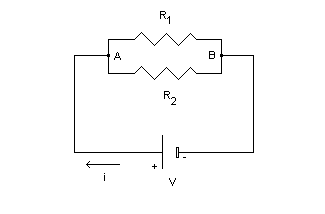
\includegraphics[width=\linewidth]{parallelo.png}
% \end{figure}

\textbf{Ai capi ($A$ e $B$) dei due resistori vi è la medesima tensione} che è quella del generatore. Questo fatto caratterizza i resistori collegati in parallelo.\\
Dentro i due resistori circoleranno correnti in generali \textbf{diverse} la cui somma, a causa del principio di conservazione della carica, uguaglierà la corrente complessiva che passa nel generatore.

Avremo: 
% ![Circui51](assets/Circui54.gif)
Le due \textbf{correnti} sono immediatamente \textbf{calcolabili}:

\begin{equation}
  i_1=\frac{V}{R_1}
\end{equation}
\begin{equation}
  i_2=\frac{V}{R_2}
\end{equation}

essendo la \textbf{tensione} ai \textbf{capi} dei due \textbf{resistori} la \textbf{stessa}, ovvero la \textbf{tensione} $V$ del \textbf{generatore}.\\
La corrente $i$ che attraversa il circuito si trova tenendo conto di tutte le resistenze. \\
\textbf{Corto circuito} $=$ \textbf{Circuito chiuso}: \textbf{resistenza prossima allo 0} quindi passa corrente.\\
% \subsubsection*{CONDENSATORE}

% Ha la capacità di immagazzinare energia elettrica tra le sue armature

% - \textbf{Circuito (interruttore) aperto} : \textbf{non passa corrente}
% - \textbf{Circuito (interruttore) chiuso} : \textbf{passa corrente}

% - \textbf{Condensatore scarico} + \textbf{circuito chiuso} (interruttore chiuso, quindi passa corrente) -> passa corrente attraverso il Condensatore \textbf{finché} esso non sarà \textbf{carico}.
% - \textbf{Condensatore carico} : \textbf{non passa} corrente (si comporta come un circuito aperto)

% \subsubsection*{INDUTTORE}

% è il \textbf{duale} del Condensatore.
\pagebreak

\subsubsection{STAZIONAREITÀ}
\begin{itemize}
  \item \textbf{Condensatore} non passa corrente
  \item \textbf{Induttore} è \textbf{corto circuito} / \textbf{circuito chiuso} quindi passa corrente.
\end{itemize}
\subsubsection{NON STAZIONAREITÀ}
\begin{itemize}
  \item \textbf{Condensatore} 
  \begin{itemize}
    \item in \textbf{scarica} passa corrente (diventa un generatore)
    \item in \textbf{carica} passa corrente
    \item in \textbf{parallelo} con Resistore: resistore si \textbf{annulla}
  \end{itemize}
  \item \textbf{Induttore}: \textbf{non passa corrente} (circuito aperto) 
\end{itemize}

\end{document}